\documentclass[12pt]{article}
%%%%%%%%%%%%%%%%%%%%%%%%%%%%%
% Preambulo
\usepackage[lmargin=2cm,rmargin=2cm,top=1.5cm,
bottom=2cm]{geometry}
\usepackage[T1]{fontenc}
\usepackage[utf8]{inputenc}
\usepackage[spanish,es-tabla]{babel}
\parindent=0cm %modificar tamaño de sangria 
\usepackage{amsmath}
\usepackage{amssymb,amsfonts,latexsym,cancel}
\usepackage{graphicx}
\usepackage{epstopdf}
\usepackage{float}
\usepackage{subfigure}
\usepackage{array}
\usepackage{longtable}
\newcolumntype{E}{>{$}c<{$}}
\setcounter{MaxMatrixCols}{40}
\usepackage{bm}
\usepackage{fancyhdr}

\pagestyle{fancy}
\fancyhead{}
\fancyhead[C]{Titulo del articulo}
\fancyfoot{}
\fancyfoot[R]{\thepage}
\fancyfoot[L]{Héctor Misael}
\renewcommand{\headrulewidth}{0pt}
%%%%%%%%%%%%%%%%%%%%%%%%%%%%%%%%%%%%%%
%% Paquetes o configuración nueva 
%---->%%%%%%%%%%%%%%%%%%%%%%%%%%%%%%%%
\usepackage[sc]{mathpazo}
\usepackage{multicol}
\usepackage{titling}
\usepackage{titlesec}
\usepackage[colorlinks = true,
           linkcolor = blue,
           urlcolor = black,
           citecolor = blue ]{hyperref}
\renewcommand{\thesection}{\Roman{section}}
\renewcommand{\thesubsection}{\roman{subsection}}
\titleformat{\section}[block]{\bfseries\centering}{\thesection.}{1mm}{}
\titleformat{\subsection}[block]{\bfseries\centering}{\thesubsection.}{1mm}{}
%% Titulo del articulo
%%
%%------------------------------------------------
\setlength{\droptitle}{-4.5\baselineskip}
\title{{\Huge\textbf{Segundo Ejemplo}}}
\author{\textsc{Héctor Misael}
\thanks{Información relacionada con el autor}\\[0.2cm]
\normalsize Universidad de Guadalajara \\
\normalsize 
\href{mailto:hectormisael.bn@gmail.com}{hectormisael.bn@gmail.com}
}
%---->%%%%%%%%%%%%%%%%%%%%%%%%%%%%%%%%
\begin{document}
\maketitle
\renewcommand{\contentsname}{Contenido}
\tableofcontents

\begin{abstract}
Se presenta una introducción a los siguientes temas El producto de dos binomios conjugados es igual al cuadrado de el primer término menos el cuadrado del segundo término.
Se presenta una introducción a los siguientes temas El producto de dos binomios conjugados es igual al cuadrado de el primer término menos el cuadrado del segundo término.
Se presenta una introducción a los siguientes temas El producto de dos binomios conjugados es igual al cuadrado de el primer término menos el cuadrado del segundo término.
Se presenta una introducción a los siguientes temas El producto de dos binomios conjugados es igual al cuadrado de el primer término menos el cuadrado del segundo término.
\end{abstract}

\begin{multicols}{2}
\section{Primera sección}
Se presenta una introducción a los siguientes\footnote{primera nota} temas El producto de dos binomios conjugados es igual al cuadrado de el primer término menos el cuadrado del segundo término.
Se presenta una introducción a los siguientes temas El producto de dos binomios conjugados es igual al cuadrado de el primer término menos el cuadrado del segundo término.
Se presenta una introducción a los siguientes temas El producto de dos binomios conjugados es igual al cuadrado de el primer término menos el cuadrado del segundo término.
Se presenta una introducción a los siguientes temas El producto de dos binomios conjugados es igual al cuadrado de el primer término menos el cuadrado del segundo término.
\subsection{Primera subsección}
\begin{figure*}[ht]
\centering
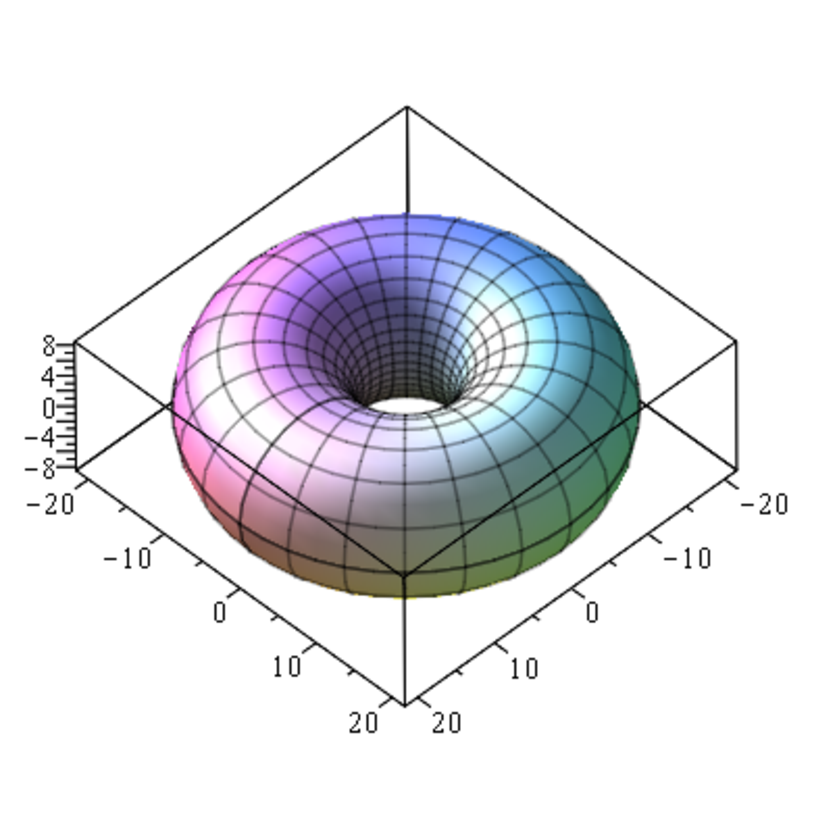
\includegraphics[scale=0.5]{figuras/fig3d_3}
\caption{primer figura*}
\end{figure*}
Se presenta una introducción a los siguientes temas El producto de dos binomios conjugados es igual al cuadrado de el primer término menos el cuadrado del segundo término.
\section{Segunda sección}
\begin{figure}[H]
\centering
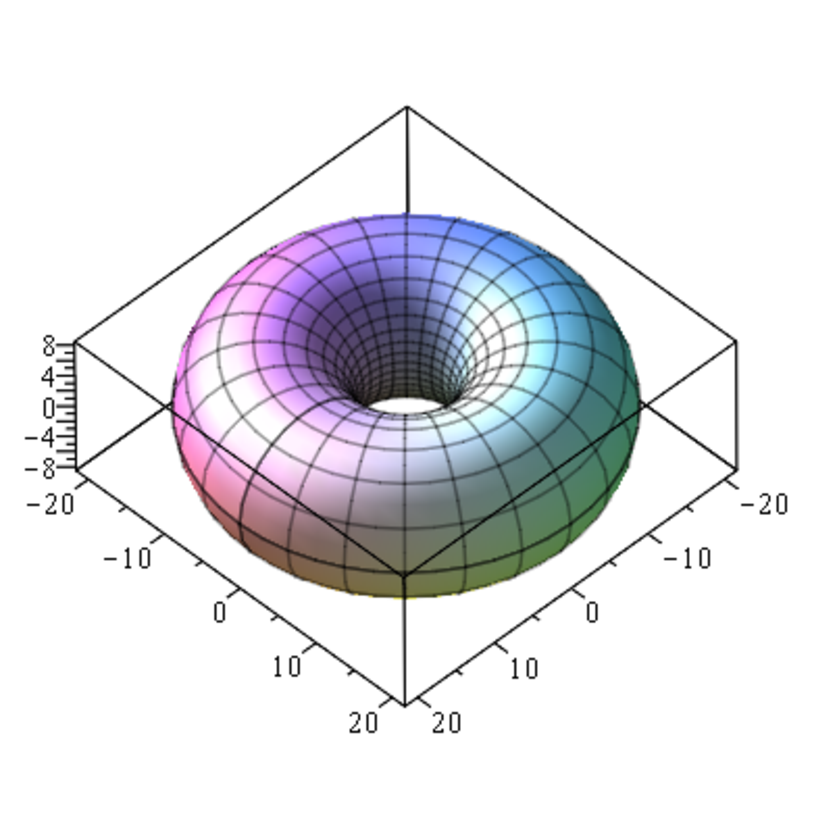
\includegraphics[scale=0.5]{figuras/fig3d_3}
\caption{primer figura}
\end{figure}
Se presenta una introducción a los siguientes temas El producto de dos binomios conjugados es igual al cuadrado de el primer término menos el cuadrado del segundo término.
Se presenta una introducción a los siguientes temas El producto de dos binomios conjugados es igual al cuadrado de el primer término menos el cuadrado del segundo término.
Se presenta una introducción a los siguientes temas El producto de dos binomios conjugados es igual al cuadrado de el primer término menos el cuadrado del segundo término.
\section{Tercera sección}
Se presenta una introducción\footnote{segunda nota} a los siguientes temas El producto de dos binomios conjugados es igual al cuadrado de el primer término menos el cuadrado del segundo término.
Se presenta una introducción a los siguientes temas El producto de dos binomios conjugados es igual al cuadrado de el primer término menos el cuadrado del segundo término.
Se presenta una introducción a los siguientes temas El producto de dos binomios conjugados es igual al cuadrado de el primer término menos el cuadrado del segundo término.
\subsection{Segunda subsección}
\begin{figure*}[hb]
\centering
\subfigure[uno]{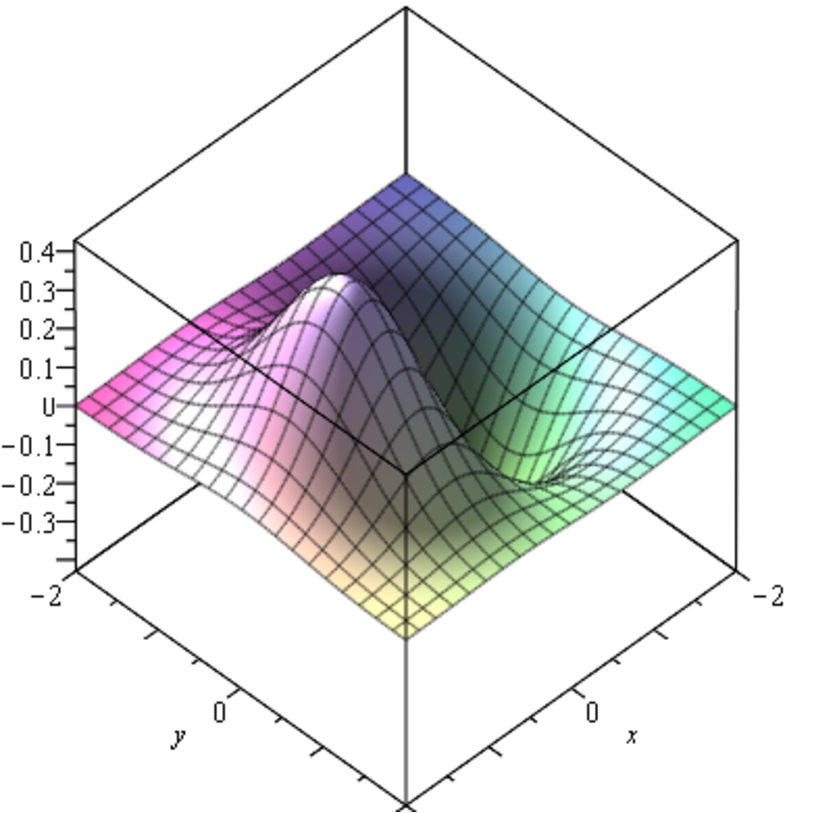
\includegraphics[scale=0.4]{figuras/fig3d_1}} \hspace{0.3cm}
\subfigure[dos]{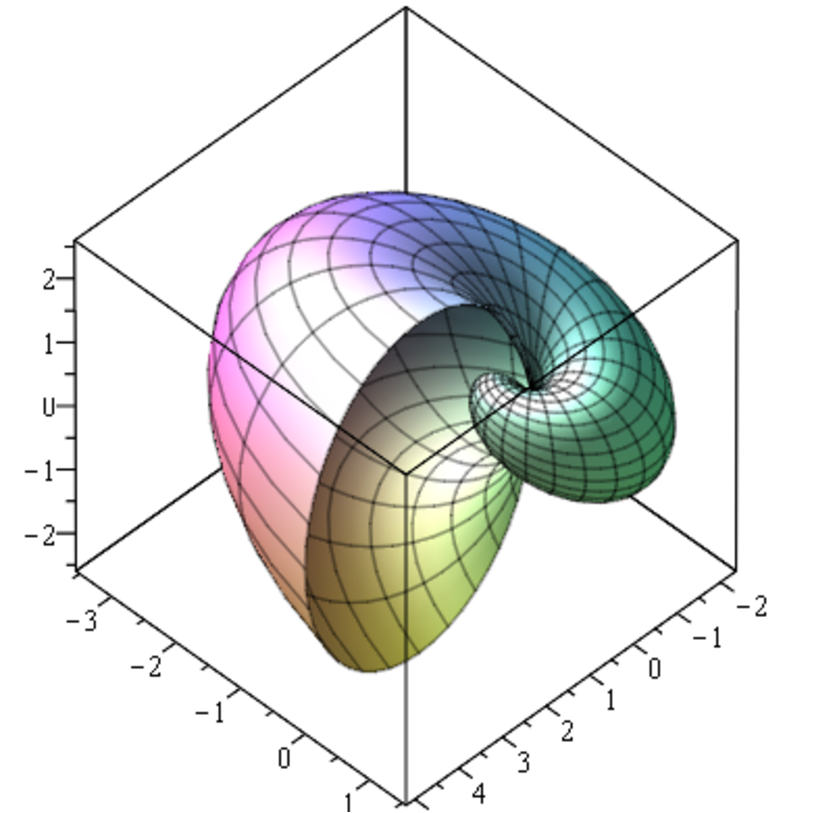
\includegraphics[scale=0.4]{figuras/fig3d_2}}
\caption{Grafícas multiples*}
\end{figure*}

\begin{table*}[ht]
\centering
\begin{tabular}{|c|c|c|}
\hline
elemento uno & elemento dos & elemento tres \\ \hline
elemento uno & elemento dos & elemento tres \\ \hline
elemento uno & elemento dos & elemento tres \\ \hline
\end{tabular}
\caption{figura en ancho de pagina}
\end{table*}
Se presenta una introducción a los siguientes temas El producto de dos binomios conjugados es igual al cuadrado de el primer término menos el cuadrado del segundo término.
\begin{table}[H]
\centering
\begin{tabular}{|c|c|c|}
\hline
elemento uno & elemento dos & elemento tres \\ \hline
elemento uno & elemento dos & elemento tres \\ \hline
elemento uno & elemento dos & elemento tres \\ \hline
\end{tabular}
\caption{figura en una columna}
\end{table}
Se presenta una introducción a los siguientes temas El producto de dos binomios conjugados es igual al cuadrado de el primer término menos el cuadrado del segundo término.
Se presenta una introducción a los siguientes temas El producto de dos binomios conjugados es igual al cuadrado de el primer término menos el cuadrado del segundo término.
\subsection{Tercera subsección}
Se presenta una introducción a los siguientes temas El producto de dos binomios conjugados es igual al cuadrado de el primer término menos el cuadrado del segundo término.
Se presenta una introducción a los siguientes temas El producto de dos binomios conjugados es igual al cuadrado de el primer término menos el cuadrado del segundo término.
Se presenta una introducción a los siguientes temas El producto de dos binomios conjugados es igual al cuadrado de el primer término menos el cuadrado del segundo término.
\subsection{Cuarta subsección}
Se presenta una introducción a los siguientes temas El producto de dos binomios conjugados es igual al cuadrado de el primer término menos el cuadrado del segundo término.
Se presenta una introducción a los siguientes temas El producto de dos binomios conjugados es igual al cuadrado de el primer término menos el cuadrado del segundo término.
Se presenta una introducción a los siguientes temas El producto de dos binomios conjugados es igual al cuadrado de el primer término menos el cuadrado del segundo término.
\end{multicols}
\newpage
\begin{thebibliography}{99}
\bibitem{Nombre1} Articulo o libro 1, Autor 1, Año de referencia 1.
\bibitem{Nombre2} Articulo o libro 1, Autor 1, Año de referencia 1.
\bibitem{Nombre3} Articulo o libro 1, Autor 1, Año de referencia 1.
\bibitem{Nombre4} Articulo o libro 1, Autor 1, Año de referencia 1.
\bibitem{Nombre5} Articulo o libro 1, Autor 1, Año de referencia 1.
\bibitem{Nombre6} Articulo o libro 1, Autor 1, Año de referencia 1.
\end{thebibliography}
\end{document}